% !TEX root = frenetic_programmers_guide.tex

\chapter{SDN Development Tools}

\section{Tmux}

Tmux stands for \emph{terminal multiplexor}, and it's indispensible for all kinds of multi-program development.
It's a Window Manager for the command line, of sorts.
With tmux you can split the screen into \emph{panes}, each of which can run a different shell.

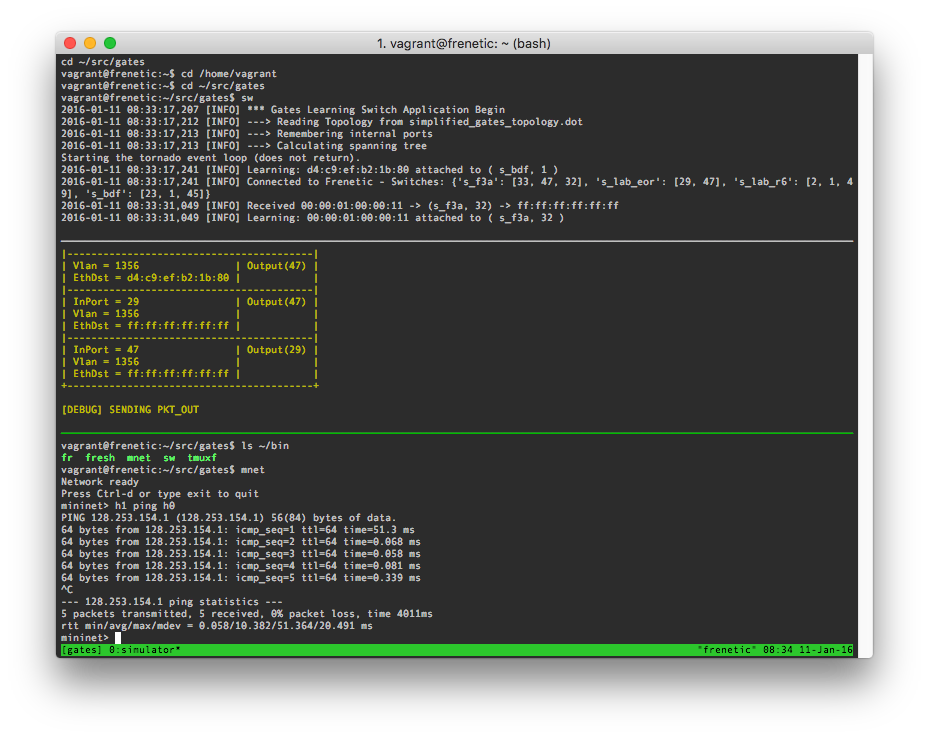
\includegraphics[scale=0.4]{tmux_example}

In Frenetic development, it's helpful to run tmux with at least 3 panes, which you can see in the example above:

\begin{enumerate}
\item One pane runs your network application, e.g. \netkat{python repeater.py}
\item One pane runs Frenetic, e.g. \netkat{frenetic http-server --verbosity debug}
\item One pane runs Mininet
\end{enumerate}

Tmux is very personalizable and configurable.  
But if you haven't used tmux before, here is a good setup to get you started.

\begin{enumerate}
\item Install tmux on Frenetic-vm with \netkat{sudo apt-get install tmux}
\item Create a file in your home directory, ./tmux.conf with the line \netkat{set -g prefix C-a}.  
This maps the tmux prefix key to \Ctrl+\keystroke{A}, which is much easier to reach than the default 
\Ctrl+\keystroke{B}
\item Type \netkat{tmux} to start.
\end{enumerate}

\Ctrl+\keystroke{A} is called the \emph{prefix key}, and we'll denote it as \keystroke{Prefix} below. 
Because you will be typing the prefix a lot, it's really helpful to map your \keystroke{Caps Lock} key to \Ctrl, if
you haven't already done so.  
On a Mac, for example, you can go to Apple Menu $\rightarrow$ System Preferences $\rightarrow$ Keyboard 
$\rightarrow$ Keyboard Tab $\rightarrow$ Modifier Keys and select Control for Caps Lock.

Once there, you can use the following key combinations:

\begin{itemize}
\item \keystroke{Prefix} \keystroke{=} splits the pane at the cursor into two panes: one above the cursor and one below.  
You can split existing panes as many times as you want, all the way down to panes with one line (which are probably
not very useful).   
\item \keystroke{Prefix} \UArrow moves the cursor to the pane above.
(If you're on the top pane already, the cursor moves to the bottom-most pane.)
\item \keystroke{Prefix} \DArrow moves the cursor to the pane below.
(If you're on the bottom pane already, the cursor moves to the top-most pane.)
\item \keystroke{Prefix} \keystroke{Z} zooms the current pane, so that it takes up the entire window. 
The other panes continue to run, even though they're not visible.
Pressing \keystroke{Prefix} \keystroke{Z} again unzooms the window.  
\item \keystroke{Prefix} \keystroke{D} detaches from the Tmux session.  
You can start it up again later, even after having logged off the Frenetic VM, by using 
\netkat{tmux attach}.
\end{itemize}

Because tmux operates outside the normal window manager realms, you can no longer scroll up or down
in a pane using scroll bars.  
But tmux has a scrolling mechanism inside itself which scrolls panes independently.  

\begin{itemize}
\item \keystroke{Prefix}, \keystroke{[} enters scroll mode.  
You can see a cursor position status at the top right hand corner of the pane: 67/900 means you're
on line 67 of 900 lines in the pane.   
\item once in scroll mode:
\begin{itemize}
\item \UArrow moves the cursor one line up.
\item \DArrow moves the cursor one line down.
\item \PgUp moves the cursor one page up.
\item \PgDown moves the cursor one page down.
\item\Esc leaves scroll mode and scrolls all the way down to the bottom
\end{itemize}
\end{itemize}

If you end up doing the same keystrokes each time you start up an SDN session, you can automate it
with tmuxinator software.

The book \citet{hogan:tmux} is a great introduction and reference to tmux.  

\section{Open VSwitch Utilities}

\section{TCPDump}
 \label{sdn_development_tools:tcpdump}

\section{Mininet Network Modelling}

